% Options for packages loaded elsewhere
\PassOptionsToPackage{unicode}{hyperref}
\PassOptionsToPackage{hyphens}{url}
\PassOptionsToPackage{dvipsnames,svgnames,x11names}{xcolor}
%
\documentclass[
]{agujournal2019}

\usepackage{amsmath,amssymb}
\usepackage{iftex}
\ifPDFTeX
  \usepackage[T1]{fontenc}
  \usepackage[utf8]{inputenc}
  \usepackage{textcomp} % provide euro and other symbols
\else % if luatex or xetex
  \usepackage{unicode-math}
  \defaultfontfeatures{Scale=MatchLowercase}
  \defaultfontfeatures[\rmfamily]{Ligatures=TeX,Scale=1}
\fi
\usepackage{lmodern}
\ifPDFTeX\else  
    % xetex/luatex font selection
\fi
% Use upquote if available, for straight quotes in verbatim environments
\IfFileExists{upquote.sty}{\usepackage{upquote}}{}
\IfFileExists{microtype.sty}{% use microtype if available
  \usepackage[]{microtype}
  \UseMicrotypeSet[protrusion]{basicmath} % disable protrusion for tt fonts
}{}
\makeatletter
\@ifundefined{KOMAClassName}{% if non-KOMA class
  \IfFileExists{parskip.sty}{%
    \usepackage{parskip}
  }{% else
    \setlength{\parindent}{0pt}
    \setlength{\parskip}{6pt plus 2pt minus 1pt}}
}{% if KOMA class
  \KOMAoptions{parskip=half}}
\makeatother
\usepackage{xcolor}
\setlength{\emergencystretch}{3em} % prevent overfull lines
\setcounter{secnumdepth}{5}
% Make \paragraph and \subparagraph free-standing
\ifx\paragraph\undefined\else
  \let\oldparagraph\paragraph
  \renewcommand{\paragraph}[1]{\oldparagraph{#1}\mbox{}}
\fi
\ifx\subparagraph\undefined\else
  \let\oldsubparagraph\subparagraph
  \renewcommand{\subparagraph}[1]{\oldsubparagraph{#1}\mbox{}}
\fi


\providecommand{\tightlist}{%
  \setlength{\itemsep}{0pt}\setlength{\parskip}{0pt}}\usepackage{longtable,booktabs,array}
\usepackage{calc} % for calculating minipage widths
% Correct order of tables after \paragraph or \subparagraph
\usepackage{etoolbox}
\makeatletter
\patchcmd\longtable{\par}{\if@noskipsec\mbox{}\fi\par}{}{}
\makeatother
% Allow footnotes in longtable head/foot
\IfFileExists{footnotehyper.sty}{\usepackage{footnotehyper}}{\usepackage{footnote}}
\makesavenoteenv{longtable}
\usepackage{graphicx}
\makeatletter
\def\maxwidth{\ifdim\Gin@nat@width>\linewidth\linewidth\else\Gin@nat@width\fi}
\def\maxheight{\ifdim\Gin@nat@height>\textheight\textheight\else\Gin@nat@height\fi}
\makeatother
% Scale images if necessary, so that they will not overflow the page
% margins by default, and it is still possible to overwrite the defaults
% using explicit options in \includegraphics[width, height, ...]{}
\setkeys{Gin}{width=\maxwidth,height=\maxheight,keepaspectratio}
% Set default figure placement to htbp
\makeatletter
\def\fps@figure{htbp}
\makeatother
% definitions for citeproc citations
\NewDocumentCommand\citeproctext{}{}
\NewDocumentCommand\citeproc{mm}{%
  \begingroup\def\citeproctext{#2}\cite{#1}\endgroup}
\makeatletter
 % allow citations to break across lines
 \let\@cite@ofmt\@firstofone
 % avoid brackets around text for \cite:
 \def\@biblabel#1{}
 \def\@cite#1#2{{#1\if@tempswa , #2\fi}}
\makeatother
\newlength{\cslhangindent}
\setlength{\cslhangindent}{1.5em}
\newlength{\csllabelwidth}
\setlength{\csllabelwidth}{3em}
\newenvironment{CSLReferences}[2] % #1 hanging-indent, #2 entry-spacing
 {\begin{list}{}{%
  \setlength{\itemindent}{0pt}
  \setlength{\leftmargin}{0pt}
  \setlength{\parsep}{0pt}
  % turn on hanging indent if param 1 is 1
  \ifodd #1
   \setlength{\leftmargin}{\cslhangindent}
   \setlength{\itemindent}{-1\cslhangindent}
  \fi
  % set entry spacing
  \setlength{\itemsep}{#2\baselineskip}}}
 {\end{list}}
\usepackage{calc}
\newcommand{\CSLBlock}[1]{\hfill\break\parbox[t]{\linewidth}{\strut\ignorespaces#1\strut}}
\newcommand{\CSLLeftMargin}[1]{\parbox[t]{\csllabelwidth}{\strut#1\strut}}
\newcommand{\CSLRightInline}[1]{\parbox[t]{\linewidth - \csllabelwidth}{\strut#1\strut}}
\newcommand{\CSLIndent}[1]{\hspace{\cslhangindent}#1}

\usepackage{booktabs}
\usepackage{longtable}
\usepackage{array}
\usepackage{multirow}
\usepackage{wrapfig}
\usepackage{float}
\usepackage{colortbl}
\usepackage{pdflscape}
\usepackage{tabu}
\usepackage{threeparttable}
\usepackage{threeparttablex}
\usepackage[normalem]{ulem}
\usepackage{makecell}
\usepackage{xcolor}
\usepackage{url} %this package should fix any errors with URLs in refs.
\usepackage{lineno}
\usepackage[inline]{trackchanges} %for better track changes. finalnew option will compile document with changes incorporated.
\usepackage{soul}
\linenumbers
\makeatletter
\@ifpackageloaded{caption}{}{\usepackage{caption}}
\AtBeginDocument{%
\ifdefined\contentsname
  \renewcommand*\contentsname{Table of contents}
\else
  \newcommand\contentsname{Table of contents}
\fi
\ifdefined\listfigurename
  \renewcommand*\listfigurename{List of Figures}
\else
  \newcommand\listfigurename{List of Figures}
\fi
\ifdefined\listtablename
  \renewcommand*\listtablename{List of Tables}
\else
  \newcommand\listtablename{List of Tables}
\fi
\ifdefined\figurename
  \renewcommand*\figurename{Figure}
\else
  \newcommand\figurename{Figure}
\fi
\ifdefined\tablename
  \renewcommand*\tablename{Table}
\else
  \newcommand\tablename{Table}
\fi
}
\@ifpackageloaded{float}{}{\usepackage{float}}
\floatstyle{ruled}
\@ifundefined{c@chapter}{\newfloat{codelisting}{h}{lop}}{\newfloat{codelisting}{h}{lop}[chapter]}
\floatname{codelisting}{Listing}
\newcommand*\listoflistings{\listof{codelisting}{List of Listings}}
\makeatother
\makeatletter
\makeatother
\makeatletter
\@ifpackageloaded{caption}{}{\usepackage{caption}}
\@ifpackageloaded{subcaption}{}{\usepackage{subcaption}}
\makeatother
\ifLuaTeX
  \usepackage{selnolig}  % disable illegal ligatures
\fi
\usepackage{bookmark}

\IfFileExists{xurl.sty}{\usepackage{xurl}}{} % add URL line breaks if available
\urlstyle{same} % disable monospaced font for URLs
\hypersetup{
  pdftitle={Modeling Disability-Adjusted Life Years for Policy and Decision Analysis},
  pdfkeywords={Cost-Effectiveness Analysis, Microsimulation, Discrete
Event Simulation, Markov Cohort Models},
  colorlinks=true,
  linkcolor={blue},
  filecolor={Maroon},
  citecolor={Blue},
  urlcolor={Blue},
  pdfcreator={LaTeX via pandoc}}

\journalname{Citation title}

\draftfalse

\begin{document}
\title{Modeling Disability-Adjusted Life Years for Policy and Decision
Analysis}

\authors{}




\begin{abstract}
This study outlines a methodological framework for joint modeling of
Disability- and Quality-Adjusted Life Year outcomes.
\end{abstract}

\section*{Plain Language Summary}
Modeling Disability-Adjusted Life Years for Policy and Decision Analysis



\subsection{Introduction}\label{sec-introduction}

\textsubscript{Source:
\href{https://graveja0.github.io/dalys/index.qmd.html}{Article
Notebook}}

Disability-adjusted life years (DALYs) measure disease burden in a
population. Conceptualized in the Global Burden of Disease (GBD) study
(C. J. Murray \& Lopez, 1997), DALYs quantify the total sum of years of
life lost due to disability attributable to a disease (YLD), plus years
of life lost to premature mortality from the disease (YLL; i.e., DALY =
YLD + YLL).

In addition to their role in describing levels and trends in disease
burdens worldwide, DALYs are a primary health outcome in evaluations of
health interventions in low- and middle-income countries (LMICs). In
these settings, resource allocation decisions are guided by modeled
assessments of the incremental costs per DALY averted under alternative
(often competing) strategies to improve population health.\footnote{The
  adoption of DALYs over other common health outcomes in health
  economics (e.g., quality-adjusted life years, or QALYs) stems from
  several practical and theoretical considerations. See Feng et al.
  (2020) and Wilkinson et al. (2016) for futher discussion.}

Despite the prominent role of DALYs in global health policy, scant
methodological guidance is available for adapting and/or structuring
decision analytic models for DALY outcomes. This methodological gap has
its roots in health economics education, where textbooks and training
exercises focus almost exclusively on Quality-Adjusted Life Year (QALY)
outcomes---the primary health outcome used for health technology
assessments (HTAs) and policy decisionmaking in high-income countries
(HICs). DALYs differ from QALYs in important and model-relevant
respects, including the use of reference life tables to calculate YLLs
and standardized disability weights to calculate YLDs.\footnote{In
  contrast, QALYs are calculated based on utility weights derived from
  general and patient surveys. See Feng et al. (2020) and Wilkinson et
  al. (2016) for futher discussion.} To the extent DALY-specific
modeling considerations are taught, they are often considered in
isolation and without a firm methodological grounding in \emph{how} one
might structure a model to measure DALY outcomes.

As a consequence, and in practice, health economic applications often
resort to shortcuts and other ``hacks'' for calculating DALYs. For
example, practitioners may simply estimate a ``QALY-like'' DALY that is
based on a diseased state occupancy payoff of one minus the disability
weight. Other approaches define a diseased-state payoff using the
disability weight as an estimate of YLDs, and accumulate person-years in
an absorbing death state (due to disease) as an estimate of YLLs. As
this study will show, these shortcuts do not provide an accurate
representation of DALY levels in a population.

This tutorial outlines a framework for direct incorporation of DALY
outcomes in common decision modeling environments. Our primary focus is
on discrete-time Markov cohort models---however, our framework extends
directly to microsimulation and is also easily adapted for continuous
time discrete event simulation (DES) models. As such, our study provides
a comprehensive roadmap for incorporating DALY outcomes into common
decision modeling frameworks.

To maintain consistency within the literature, we build on an existing
didactic disease progression model (Alarid-Escudero et al., 2023). The
underlying discrete time Markov cohort model is time homogeneous---that
is, transition probabilities do not vary as a function of age/time in
model. However, our methods and code are developed to accomodate
time-inhomogenous models. Finally, recognizing the wide spectrum of
experience and programming comfort level among practitioners, we offer
three approaches for modeling DALYs (beginner, intermediate and
advanced) and provide replication materials for implementing our
approaches in R and Microsoft Excel.

\subsection{Background}\label{sec-background}

This section provides background information sufficient for conceptual
understaning of DALYs and how to estimate them in a decision-analytic
model; it is not intended as a comprehensive treatment of the subject.
For extensive discussion of the history, assumptions and controversies
around DALYs, see TK.

DALYs are the sum of two components: a morbidity component called years
lost to disability (YLD), and a premature mortality component called
years of life lost to disease (YLL) (WHO, 2013). To quantify YLDs,
conditions are assigned disability weights (\(D\)) ranging from zero to
one, with zero representing the absence of the condition and one
representing the highest burden a condition can inflict. Disability
weights are elicited from expert panels, are standardized across
geographies, and are routinely updated and published as part of the GBD
(WHO, 2013).

For a given condition \(c\), YLDs are defined as the condition's
disability weight multiplied by the average number of years a person
lives with the disease (\(L_c\)):

\begin{equation}\phantomsection\label{eq-yld1}{
YLD(c) = D_c \cdot L_c
}\end{equation}

YLLs are determined by a loss function, which is typically defined as
the number of years lost to premature mortality at age \(a\). This value
is often taken directly from a life table that provides information on
remaining life expectancy (\(Ex(a)\)) at a given age.

\begin{equation}\phantomsection\label{eq-yll1}{
YLL(a)= Ex(a)
}\end{equation} .

Choices over the specific value of remaining life expectancy will depend
on the context and research question at hand (Anand \& Reddy, 2019).
Historically, the GBD has utilized an \emph{exogenous}, external
reference life table based on the maximum potential life span among
humans (Global Burden of Disease Collaborative Network, 2021; WHO,
2013). More recent GBD estimates draw on reference life tables based on
the lowest observed age-specific mortality rates among geographies with
populations over 5 million in 2016 (Global Burden of Disease
Collaborative Network, 2021).

Finally, DALYS are simply the sum of these two components:

\begin{equation}\phantomsection\label{eq-daly}{
DALY(c,a) = YLD(c) + YLL(a)
}\end{equation}

\subsubsection{Discounting}\label{discounting}

In the original GBD study, additional age-weighting and time discounting
practices were applied to DALY calculations (C. J. Murray \& Lopez,
1997). These methods respectively weighted the burden of illness more
during adulthood than early childhood and old age, and valued present
health over future years of illness by discounting YLD and YLL measures
by 3\% per year. From 2010 onwards, both practices were discontinued to
make the DALY a more descriptive measure (WHO, 2013).

While the GBD no longer uses age and time discounting, the World Health
Organization's Choosing Interventions that are Cost-Effective
(WHO-CHOICE) program recommends consideration of time discounting of
health outcomes (Bertram et al., 2021; C. J. L. Murray et al., 2020). We
therefore adopt the WHO-CHOICE recommendation and include discounting in
our DALY modeling approach.\footnote{Practitioners who do not wish to
  discount DALY outcomes can simply set the annual discount rate \(r\)
  to zero.} We do, however, maintain the continuous-time discounting
used in the original GBD DALY equations---which differs slightly from
the more common use of discrete time discounting in Markov cohort
models.

For an annual discount rate \(r\), for condition \(c\), and at age
\(a\), the equation for YLDs is,

\begin{equation}\phantomsection\label{eq-yld}{
YLD(c) = D_c  \left ( \frac{1}{r}\left(1-e^{-r(L_c) }\right) \right ).
}\end{equation}

Similarly, YLLs are calculated as,

\begin{equation}\phantomsection\label{eq-yll}{
YLL(a)= \frac{1}{r}\left(1-e^{-r Ex(a)}\right).
}\end{equation}

It is important to note that the discounting shown in
Equation~\ref{eq-yld} and Equation~\ref{eq-yll} yield the present value
of YLD and YLL outcomes at a single point in time, when the duration of
disease (\(L_c\)) and time of death from disease (\(a\)) are known. For
a decision model where not all cohort members start off ill, that point
in time very likely occurs at some point after the baseline period---and
different illness durations and death times will, of course, occur
across individuals in a modeled cohort. As such, to be consistent with
standard practice with WHO-CHOICE, we must discount YLL and YLD outcomes
further---all the way back to the baseline (time \(t=0\)) period. This
additional discounting step will become apparent in
Section~\ref{sec-outcomes} below.

\subsection{Model Overview}\label{sec-overview}

We build on an existing progressive disease model in which healthy
individuals develop a disease with two health states (``Sick'' and
``Sicker''; Alarid-Escudero et al. (2023)). Individuals can also
transition to an absorbing death state due to causes unrelated to the
disease (i.e., ``background'' mortality), or due to disease-specific
causes.

We consider outcomes under four strategies:

\begin{itemize}
\tightlist
\item
  A \textbf{Standard of Care} strategy based on the baseline model
  parameters.
\item
  \textbf{Strategy A}, which improves the quality of life among
  individuals with the disease, but does not affect disease progression.
\item
  \textbf{Strategy B}, which reduces the rate of progression from Sick
  to Sicker by 40\%.
\item
  \textbf{Composite Strategy AB}, which jointly implements strategies A
  and B.
\end{itemize}

A state transition diagram is shown in Figure~\ref{fig-model1}. In the
figure, nodes are health states and edges depict possible transitions
among them. Edge labels are defined in terms of transition intensities
(rates). Other key model parameters are summarized in
Table~\ref{tbl-params}.

As depicted in Figure~\ref{fig-model1}, and as parameterized in our
replication code, the underlying Markov model is time homogeneous---that
is, transition rates do not vary as a function of time (e.g., the
background mortality rate is fixed and does not increase with age). This
is merely a simplification that builds on an existing time-homogeneous
model constructed for didactic purposes (Alarid-Escudero et al., 2023).
We do, however, index all formulas and other model-relevant objects with
the subscript \(t\) to allow for time-inhomogenous models. Our
replication code is also written to easily accomodate time-inhomogeneous
models.

An additional observation is worth highlighting. In our implementation
of the Sick-Sicker model, disability weights are defined as one minus
the utility weight. This is not generally the case, as DALY disability
weights are derived from expert valuations and are standardized across
countries and regions (Sassi, 2006; WHO, 2013). Utility weights, by
contrast, are often derived from general population and/or patient
samples and therefore differ across geographies (Sassi, 2006). We have
elected to parameterize our model in this way to hold this
methodological difference fixed---that is, we aim to show how
differences in methodological choices shape estimates of DALYs while
holding fixed \emph{additional} differences that might occur due to
differences in the derivation of disability and utility weights.

\begin{figure}

\centering{

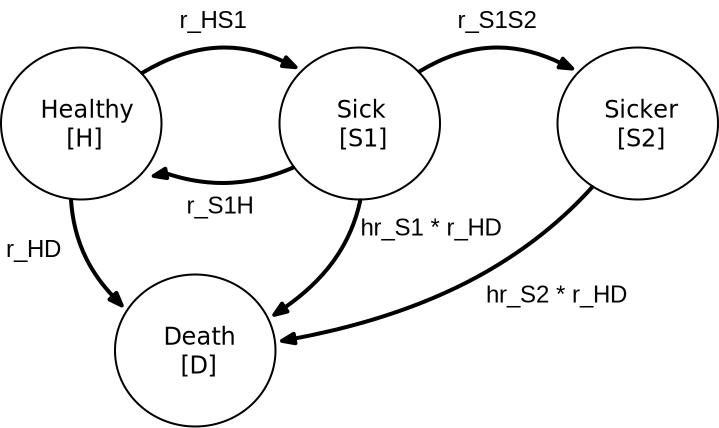
\includegraphics{index_files/mediabag/images/state-transition-diagram-1.pdf}

}

\caption{\label{fig-model1}State transition diagram for progressive
disease model}

\end{figure}%

\textsubscript{Source:
\href{https://graveja0.github.io/dalys/index.qmd.html}{Article
Notebook}}

\textsubscript{Source:
\href{https://graveja0.github.io/dalys/index.qmd.html}{Article
Notebook}}

\textsubscript{Source:
\href{https://graveja0.github.io/dalys/index.qmd.html}{Article
Notebook}}

\begin{table}

\caption{\label{tbl-params}Model Parameters}

\centering{

\centering
\begin{tabular}{l|l|l}
\hline
Parameter & Value & Description\\
\hline
v\_tx\_names & (SoC,A,B,AB)' & Treatment strategies (vector)\\
\hline
n\_tx & 4 & Number of treatment strategies\\
\hline
cycle\_correction & half-cycle & Cycle correction method\\
\hline
v\_tr\_names & (H,S1,S2)' & Transient health state names (vector)\\
\hline
v\_ab\_names & (DOC,DS)' & Absorbing health state names (vector)\\
\hline
n\_states & 5 & Total number of health states\\
\hline
horizon & 400 & Model time horizon (years)\\
\hline
r\_v\_disc\_h & 0.03 & Annual discount rate for health outcomes\\
\hline
r\_v\_disc\_c & 0.03 & Annual discount rate for cost outcomes\\
\hline
Delta\_t & 1 & Time step (cycle length; 1=annual, 1/12=monthly, etc.)\\
\hline
age0 & 25 & Age at baseline\\
\hline
r\_HS1 & 0.15 & Transition rate: healthy to sick\\
\hline
r\_S1H & 0.5 & Transition rate: sick to healthy\\
\hline
r\_S1S2 & 0.105 & Transition rate: sick to sicker\\
\hline
r\_HD & 0.002 & Transition rate: Disease-free background mortality\\
\hline
hr\_S1 & 3 & Hazard ratio: mortality from sick state\\
\hline
hr\_S2 & 10 & Hazard ratio: mortality from sicker state\\
\hline
u\_H & 1 & Utility weight: healthy [H]\\
\hline
u\_S1 & 0.75 & Utility weight: sick [S1]\\
\hline
u\_S2 & 0.5 & Utility weight: sick [S2]\\
\hline
u\_D & 0 & Utility weight: death [D]\\
\hline
dw\_S1 & 0.25 & Disability weight: sick [S1]\\
\hline
dw\_S2 & 0.5 & Disability weight: sicker [S2]\\
\hline
c\_H & 2000 & Cycle occupancy cost: healthy [H]\\
\hline
c\_S1 & 4000 & Cycle occupancy cost: sick [S1]\\
\hline
c\_S2 & 15000 & Cycle occupancy cost: sicker [S2]\\
\hline
c\_D & 0 & Cycle occupancy cost: death [D]\\
\hline
c\_trtA & 12000 & Cycle occupancy cost: treatment A [S1,S2]\\
\hline
u\_trtA & 0.95 & Utility weight: treatment A [S1]\\
\hline
dw\_trtA & 0.05 & Disbility weight: treatment A [S1]\\
\hline
c\_trtB & 12000 & Cycle occupancy cost: treatment B [S1,S2]\\
\hline
hr\_S1S2\_trtB & 0.6 & Hazard Ratio: S1 to S2 disease progression under treatment B\\
\hline
\end{tabular}

}

\end{table}%

\textsubscript{Source:
\href{https://graveja0.github.io/dalys/index.qmd.html}{Article
Notebook}}

\subsection{Transition Matrices}\label{transition-matrices}

With the model parameterized, our next step is to define the matrices
that govern transitions in the model. The state transition diagram
represented in Figure~\ref{fig-model1} is not well-suited to calculate
DALY outcomes, however. A primary reason is that transitions to the
absorbing death state capture transitions due to all causes of death. To
calculate YLLs, we need to separately track the timing and number of
deaths \emph{due to disease}.

To accommodate this need, several approaches are available. We
categorize each based on the level of experience and skill required
(beginner, intermediate, advanced):

\begin{enumerate}
\def\labelenumi{\arabic{enumi}.}
\item
  \textbf{Approach 1 (Beginner): Separate Death State}: Re-define the
  health states to include a separate cause-specific death state as
  depicted in Figure~\ref{fig-modelDS}.\footnote{In this example,
    disease-specific death rates are goverened by a hazard ratio applied
    to the background mortality rate. Because we are operating on the
    rate scale, we can separate out disease-related deaths from
    other-cause mortality by simply taking a difference in the rates.
    Other applications for prevalent conditions with high death rates,
    however, may require us to construct a cause-deleted life table to
    obtain background mortality rates that net out deaths from the
    modeled disease.} We then draw on the resulting Markov trace and use
  changes in the number of cause-specific deaths in each cycle to
  calculate YLLs.
\item
  \textbf{Approach 2 (Intermediate): Non-Markovian Trackers}: Include a
  non-Markovian transition state for cause-specific deaths in the
  transition probability matrix. This approach allows for direct
  calculation of YLD, YLL and DALY outcomes because it sidesteps the
  need to derive a separate cause-related death transition vector from
  the Markov trace (as in Approach 1).
\item
  \textbf{Approach 3 (Advanced): Markov Chain with Rewards} Define a
  block matrix Markov chain with rewards for occupancy (YLDs) and
  disease-related death transitions (YLLs) by adapting the methods in
  Caswell \& van Daalen (2021). This approach draws on matrix calculus
  and solves for expected outcomes as well as higher order moments such
  as variance and skewness.
\end{enumerate}

Each approach facilitates the design and execution of a
decision-analytic model that correctly calculates YLD, YLL, and DALY
outcomes---as well as other common outcomes such as life-years (LYs),
QALYs and costs. In practice, Approaches (1) and (2) will produce
identical results. Approach (3) draws on slightly different assumptions
on partial payoffs for partial occupancy in a cycle, but will yield
results very similar to (1) and (2). We show in
Section~\ref{sec-results} that other shortcut-based approaches
previously used in the literature---such as modeling a QALY-like DALY
and/or accumulating time in the absorbing death state---will not in
general yield similar results.

\subsubsection{Approach 1 (Beginner): Cause-Specific Death
State}\label{approach-1-beginner-cause-specific-death-state}

Under this approach, we separate out deaths from disease vs.~other
causes by defining a separate health state for cause-specific mortality;
an updated state transition diagram is shown in
Figure~\ref{fig-modelDS}.

\begin{figure}

\centering{

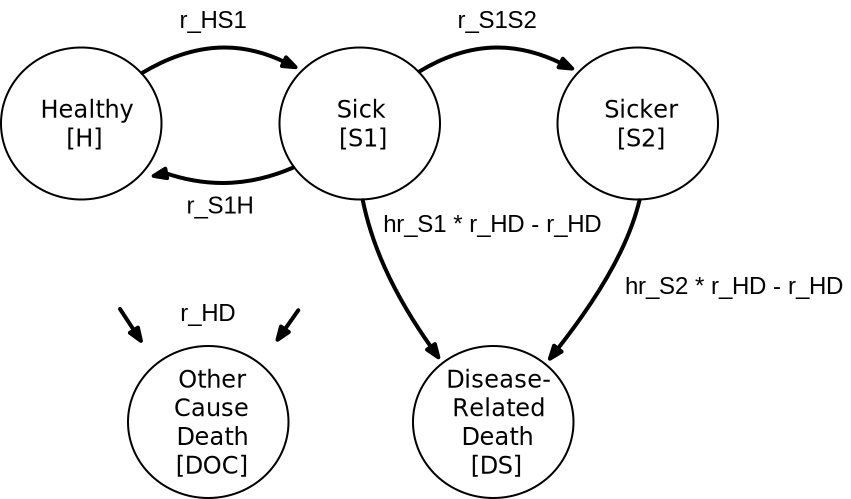
\includegraphics{index_files/mediabag/images/state-transition-diagram-2.pdf}

}

\caption{\label{fig-modelDS}State transition diagram for progressive
disease model with separate cause-specific death state}

\end{figure}%

Transitions among health states are defined in terms of continuous rates
(``intensities'') and are captured within an intensity matrix
\(\mathbf{Q}_t\),

\begin{figure}[H]

{\centering 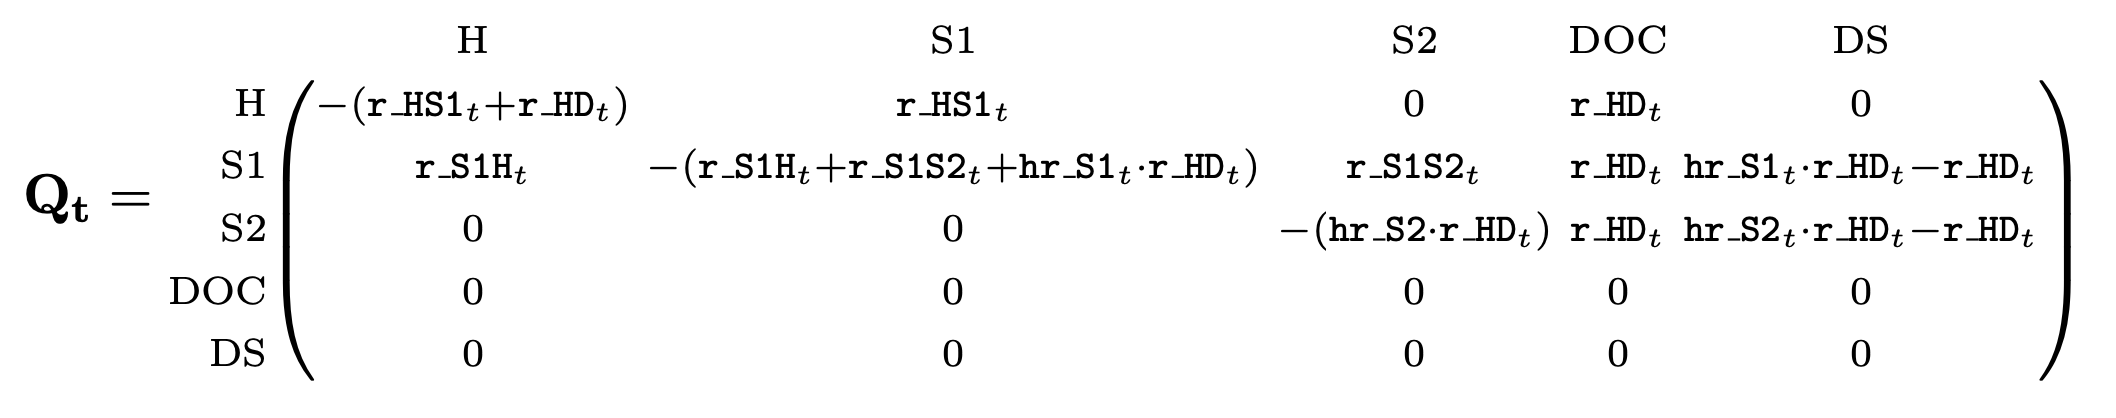
\includegraphics{images/Q_model2.png}

}

\caption{Transition Intensity Matrix for Approach 1}

\end{figure}%

Cell values in row \(i\), column \(j\) of \(\mathbf{Q}_t\) capture the
(continuous time) transition rate from health state \(i\) to health
state \(j\). \(\mathbf{Q}_t\) has diagonal elements defined as the
negative sum of the off-diagonal row values (i.e., the row sums of
\(\mathbf{Q}_t\) are zero). This ensures that the Markov model is
``closed''---that is, the total cohort size neither grows nor shrinks
over time.

We next embed the transition intensity matrix into a discrete time
transition probability matrix by taking the matrix exponential of
\(\mathbf{Q}_t\) for a defined time step (i.e., ``cycle length'')
\(\Delta t\):\footnote{In Markov theory, \(\mathbf{P}\) is called the
  ``discrete skeleton'' of the continuous model (Iosifescu, 1980). The
  conversion formula used to calculate \(mathbf{P}\) is the matrix
  analogue to the standard rate-to-probability formula commonly taught
  in health economics textbooks, i.e., \(p = 1 - e^{r\Delta t}\), where
  \(r\) is the rate and \(\Delta t\) is the time step (i.e., ``cycle
  length'').}

\begin{equation}\phantomsection\label{eq-embed}{
\mathbf{P}_t = e^{\mathbf{Q}_t\Delta t}
}\end{equation}

Embedding the Sick-Sicker model results in a transition probability
matrix \(\mathbf{P}_t\) with the following probabilities defined:

\begin{figure}[H]

{\centering 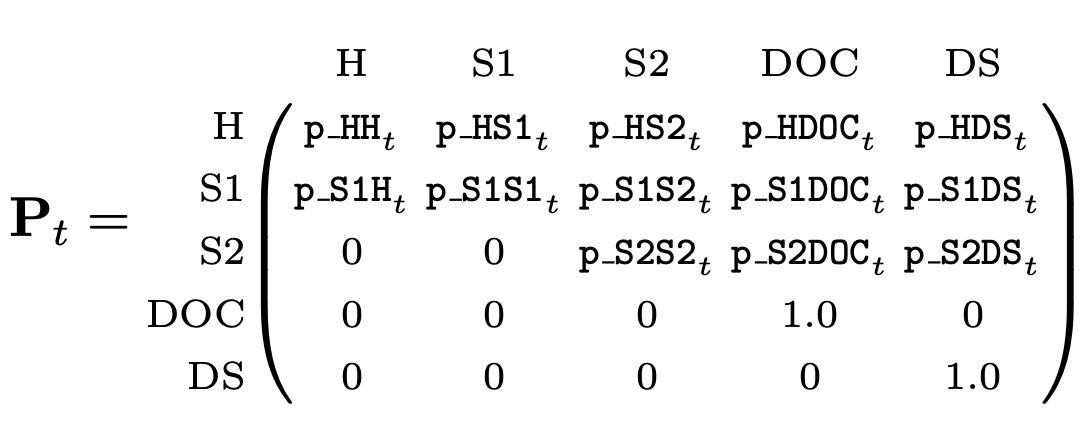
\includegraphics[width=0.6\textwidth,height=\textheight]{images/P_model2.png}

}

\caption{Transition Probability Matrix for Approach 1}

\end{figure}%

Embedding the transition probability matrix using the matrix exponential
ensures that the resulting transition probabilities capture the
underlying continuous time disease process. In particular,
\(\mathbf{P}\) will capture the probability of compound (``jumpover'')
transitions within a single cycle.\footnote{For example, in the
  continuous time rate matrix \(\mathbf{Q}_t\) above, there is a
  zero-valued rate defined for progressions from Healthy (H) to
  Disease-related death (DS), since individuals must first become ill
  before they can die from disease-related causes. However, after
  embedding, the matrix \(\mathbf{P}\) has a non-zero cycle transition
  probability from Healthy (H) to Disease-related death (DS) (i.e.,
  \(\texttt{p\_HDS}\)). This value captures the probability of a
  compound or ``jumpover'' transition from Healthy and through the Sick
  and/or Sicker state to death from disease-related causes within the
  same discrete time cycle; see Graves et al. (2021) for further
  discussion, and Iosifescu (1980) for additional
  theory.{[}\^{}comparison{]}}

\subsubsection{Approach 2 (Intermediate): Non-Markovian Tracking
States}\label{approach-2-intermediate-non-markovian-tracking-states}

Under this approach, we maintain the overall structure as depicted in
the original Figure~\ref{fig-model1}, but augment the transition
probability matrix with non-Markovian components to facilitate
accounting of disease-related deaths.\footnote{Tracking states also
  allow for accurate bookeeping for other outcomes such as costs. For
  example, if developing the disease incurs a one-time diagnosis or
  treatment cost, the compound transitions implied by the embedded
  transition probability matrix indicate that some individuals will
  transiently enter (and then exit) the Sick state in a single cycle.
  When calculating costs, practitioners may want to include a tracking
  state for the Sick state to be sure to capture these one-time costs,
  which would be masked if cost payoffs are simply multiplied by state
  occupancy at the end of each cycle (e.g., costs for individuals with a
  sojourn through the Sick state in a single cycle would not be
  accounted for).} Approach 2 offers a more generalized method that
allows practitioners to accurately account for costs and/or health
payoffs (such as YLLs) that are defined by \emph{transitions} among
health states, rather than occupancy in a health state. DALY outcomes
can also be calculated directly, without the need to derive a vector of
disease-related death transitions from the Markov trace (as required for
Approach 1).

Figure~\ref{fig-transition} shows a state transition diagram with the
tracking state added. The tracking state (shown as red nodes) simply
records transitions as cohort members move from either diseased state to
the absorbing death state due to causes related to the disease.

\begin{figure}

\centering{

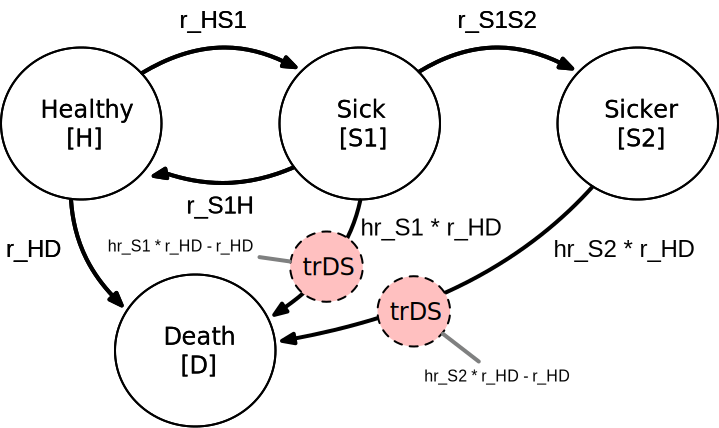
\includegraphics{index_files/mediabag/images/state-transition-diagram-3.pdf}

}

\caption{\label{fig-transition}State Transition Diagram with Transition
State (Red)}

\end{figure}%

In general, tracking states can either count the total number of
transitions that have occurred up to a given cycle (i.e., an
``accumulator'' state), or can track the total number of new transitions
that occur within a single cycle (i.e., a ``transition''
state).\footnote{More generally, accumulator and transition states can
  be defined for any number of transition types, as they are useful for
  capturing one-time costs in the model, or for for calculating other
  decision-relevant outcomes such as the total number of people who
  developed the disease or died from the disease as secondary outcomes.}
To calculate YLL outcomes we will add a transition state that records
the total number of new disease-related deaths in each cycle.

To implement Approach 2, we add a transition state row and column to the
transition intensity matrix. This transition state, called
\(\texttt{trDS}\), is included in the augmented intensity matrix
\(\mathbf{Q}_t\) below:

\begin{figure}[H]

{\centering 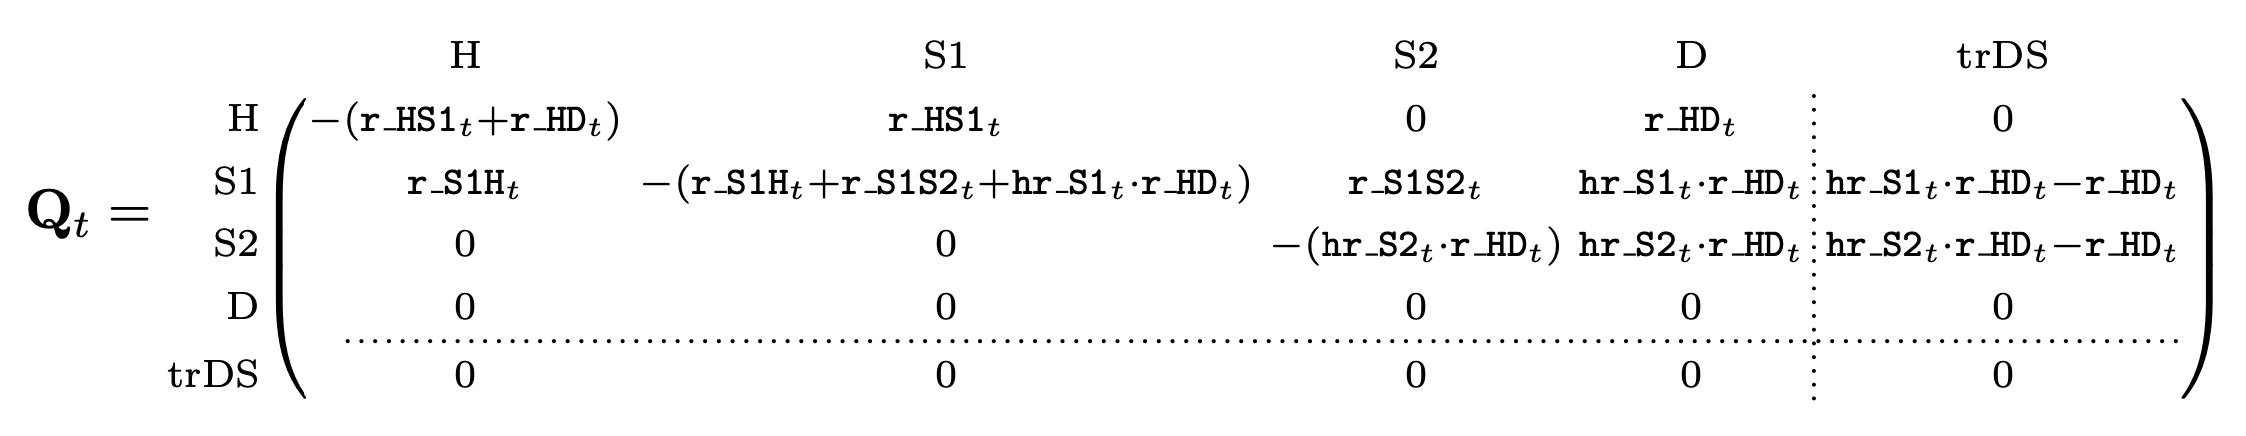
\includegraphics{images/Q_model1.png}

}

\caption{Transition intensity matrix with transition state added}

\end{figure}%

Two aspects of \(\mathbf{Q}_t\) are worth highlighting. First,
\(\mathbf{Q}_t\) is divided into a Markovian submatrix and the
non-Markovian tracking row and column. This division is made apparent
using dotted vertical and horizontal lines. Critically, the Markovian
submatrix remains closed---that is, the diagonal elements remain
unchanged so that the row sums of the submatrix remain zero, even after
the addition of the tracking column along the ``edges'' of
\(\mathbf{Q}_t\). This ensures that the Markovian submatrix can be used
to calculate state occupancy for a closed cohort that neither gains nor
loses cohort members over time.

Second, two transition intensities---from the S1 (Sick) and S2 (Sicker)
states to Death---appear in the tracking column. This ensures that
\(\texttt{trDeadDisease}\) will track all relevant transitions to death
due to the disease. Because we are operating on the rate scale, we can
net out non-disease related deaths as captured by the background
mortality rate among healthy individuals (i.e., \(\texttt{r\_HD}\)).
Other approaches might draw on cause-deleted life tables to incorporate
death transition rates that net out deaths from the disease
itself.\footnote{For an example of how to do this using Global Burden of
  Disease cause of death and life table data, see the
  \href{https://graveja0.github.io/vchem-website/blog/posts/modeling-dalys/modeling-dalys.html}{example
  here}}

As above, we obtain the transition probability matrix by embedding
\(\mathbf{Q}_t\) into the discrete time step (Equation~\ref{eq-embed}).
However, the resulting transition probability matrix treats
\(\texttt{trDS}\) as an absorbing state (i.e., individuals are retained
in the \(\texttt{trDS}\) with probability one). Using the terminology
introduced above, this absorbing state could serve as an
\textbf{accumulator} state that (in the constructed Markov trace)
records the total number of people who have died from the disease up to
any given cycle. This may be a decision-relevant health outcome to
consider on its own; indeed, so long as the Markovian submatrix remains
closed, there is no limit to the number of accumulator and/or transition
states one might add along the ``edges'' of a model.\footnote{To build
  on the example of compound ``jumpover'' transitions above, suppose an
  individual starts off healthy in a cycle, then rapidly transitions
  through the Sick and Sicker state and dies due to disease-related
  causes within the same cycle. If there is some treatment cost
  associated with being in the Sicker state, a traditional approach that
  applies cost payoffs to state occupancy at the (beginning) end of the
  cycle would miss treatment costs for this individual because they
  \emph{transition} through the Sicker state, but never occupy it at the
  beginning or end of a cycle. Adding a non-Markovian transition state
  to the model facilitates more accurate bookkeeping because the
  transition state would pick up on this transition through the Sicker
  state.}

To change \(\texttt{trDS}\) to a \textbf{transition} state, we simply
replace the absorbing probability of one in the cell
\([\texttt{trDS},\texttt{trDS}]\) with a zero. This cell-level change is
highlighted in grey in the bottom right cell of \(\mathbf{P}\) below:

\begin{figure}[H]

{\centering 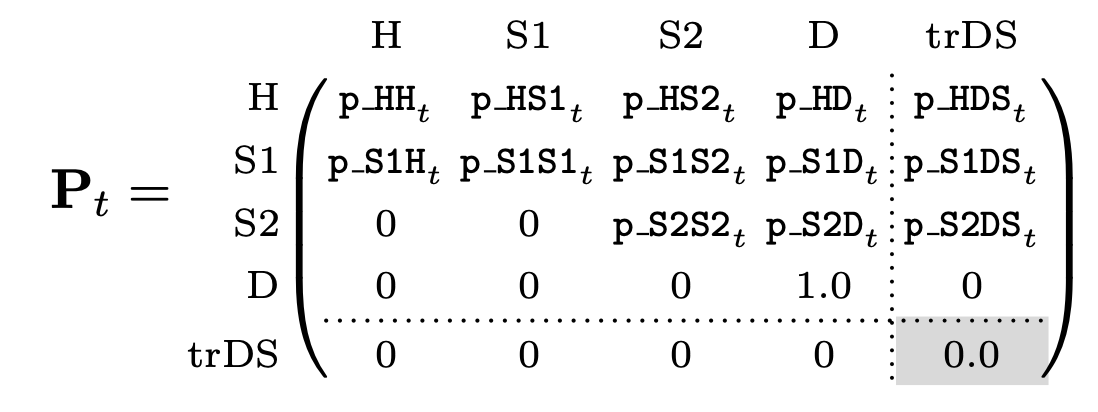
\includegraphics[width=0.6\textwidth,height=\textheight]{images/P_model1.png}

}

\caption{Transition Probability Matrix for Approach 2}

\end{figure}%

\textsubscript{Source:
\href{https://graveja0.github.io/dalys/index.qmd.html}{Article
Notebook}}

\subsubsection{Approach 3 (Advanced): Markov Chain With
Rewards}\label{approach-3-advanced-markov-chain-with-rewards}

Our final approach adapts methods from mathematical demography to
estimate YLD, YLL and DALY outcomes (Caswell \& van Daalen,
2021).\footnote{The method also easily accomodates other common outcomes
  such as QALYs and costs.} This approach requires a separate
disease-related absorbing state as shown in Figure~\ref{fig-modelDS}.
While our focus here is on expected outcomes, this method can also be
used to estimate higher order moments (e.g., variance, skewness). It is
also quite flexible and can estimate separate outcomes for any
combination of health states and age classes (e.g., disease-free
survival among those aged 40-45, etc.); see Caswell \& Zarulli (2018)
and Caswell \& van Daalen (2021) for details.

To implement Approach 3 we define some additional parameters:

\[
\begin{aligned}
\tau &= \text{Number of transient (non-absorbing) states}\\
\alpha &= \text{Number of absorbing states}\\
\omega &= \text{Number of cycles (age classes)} \\
s &= \text{Total number of states; }s=\tau\omega+\alpha \\
\mathbf{K} &= \text{vec-permutation matrix; parameters }\tau,\omega\\
\mathbf{U}_{t} &= \text{Transition matrix at time }t, \text{for }t=1,\dots,\omega\\
\mathbf{M}_{t} &= \text{Mortality matrix at time  }t, \text{for } t = 1,\dots\omega \\
\mathbf{D}_{j} &=\text{Age advancement matrix for stage }j, \text{for }j=1,\dots,\tau 
\end{aligned}
\] In the above notation, \(\mathbf{K}\) is a permutation matrix known
as the vec-permutation matrix.\footnote{See Henderson \& Searle (1981)
  and Appendix B in Caswell \& van Daalen (2021) for further
  information. A function to construct a vec-permultation matrix is
  provided within our replication code.} The matrix \(\mathbf{U}_t\)
captures transition probabilities among transient (i.e., non-absorbing)
health states, while \(\mathbf{M}_t\) contains transition probabilities
from transient health states to the absorbing (death) states.

To construct \(\mathbf{U}_t\) and \(\mathbf{M}_t\) we define transition
rate (``intensity'') matrices as in Approaches 1 and 2 above. One
important (minor) difference is that the rows in \(\mathbf{Q}_t\),
\(\mathbf{V}_t\), and \(\mathbf{S}_t\) now correspond to the final
state, while the columns correspond to the starting state; this is
essentially the transpose of the rate matrices defined for Approaches 1
and 2, where rows corresponded to the initial health state and columns
to the final health state.

The overall intensity matrix \(\mathbf{Q}_t\) is given by

\begin{equation}\phantomsection\label{eq-Qx}{
\mathbf{Q}_t=\left(\begin{array}{c|c}
\mathbf{V}_t & \mathbf{0} \\
\hline \mathbf{S}_t  & \mathbf{0}
\end{array}\right)
}\end{equation} where \(\mathbf{V}_t\) is the rate matrix for the
transitory (i.e., non-absorbing) states and \(\mathbf{S}_t\) is the rate
matrix for the absorbing states. The diagonal elements of
\(\mathbf{Q}_t\) are the negative sum of the non-diagonal column
elements, thus making the column sums of \(\mathbf{Q}_t\) zero (i.e.,
the model is ``closed'' and does not gain or lose cohort members over
time).

For the defined time step \(\Delta_t\), the discrete time transition
probability matrix \(\mathbf{P}_t\) is again obtained by taking the
matrix exponential of the intensity matrix (\(\mathbf{Q}_t\)) multipled
by the time step (\(\Delta_t\)), i.e., Equation~\ref{eq-embed}:

\[
\mathbf{P}_t =e^{\mathbf{Q}_t  \Delta t}
\]

We obtain \(\mathbf{U}_t\) and \(\mathbf{M}_t\) from the block matrix
structure of \(\mathbf{P}_t\):

\begin{equation}\phantomsection\label{eq-P3}{
\mathbf{P}_t =\left(\begin{array}{c|c}
\mathbf{U}_t  & \mathbf{0} \\
\hline \mathbf{M}_t  & \mathbf{0}
\end{array}\right)
}\end{equation}

In addition, the matrix \(\mathbf{D}_j\) defines age advancement in the
Markov chain. Borrowing from an example in Caswell \& van Daalen (2021),
if \(\omega=3\) then

\begin{equation}\phantomsection\label{eq-D}{
\mathbf{D}_j=\left(\begin{array}{ccc}
0 & 0 & 0 \\
1 & 0 & 0 \\
0 & 1 & {[1]}
\end{array}\right) \quad j=1, \ldots, \tau
}\end{equation}

In our implementation, we include the (optional) value of one in the
lower right corner; this assumes that after the last specified age, the
cohort continues to experience transitions among health states according
to the transition probabilities defined for the last age class. If this
value is zero, the model will assume that everyone dies after the last
cycle.

We next combine the transition matrices (for all age classes as defined
by discrete time cycles) together into a series of block-structured
matrices as follows:

\begin{equation}\phantomsection\label{eq-bbU}{
\mathbb{U}=\left(\begin{array}{c|c|c}
\mathbf{U}_1 & \cdots & \mathbf{0} \\
\hline & \ddots & \\
\hline \mathbf{0} & \cdots & \mathbf{U}_\omega
\end{array}\right)
}\end{equation}

\begin{equation}\phantomsection\label{eq-BBD}{
\mathbb{D}=\left(\begin{array}{c|c|c}
\mathbf{D}_1 & \cdots & \mathbf{0} \\
\hline & \ddots & \\
\hline \mathbf{0} & \cdots & \mathbf{D}_\tau
\end{array}\right)
}\end{equation}

\begin{equation}\phantomsection\label{eq-Utilde}{
\widetilde{\mathbf{U}}=\mathbf{K}^{\top} \mathbb{D} \mathbf{K} \mathbb{U} \quad \tau \omega \times \tau \omega
}\end{equation} where \(^\top\) is the transpose operator.

We also define

\begin{equation}\phantomsection\label{eq-Mtilde}{
\widetilde{\mathbf{M}}=\left(\begin{array}{lll}
\mathbf{M}_1 & \cdots & \mathbf{M}_\omega
\end{array}\right) \quad \alpha \times \tau \omega
}\end{equation}

Finally, we capture the entire Markov chain in a block transition
matrix,

\begin{equation}\phantomsection\label{eq-Ptilde}{
\widetilde{\mathbf{P}}=\left(\begin{array}{c|c}
\widetilde{\mathbf{U}} & \mathbf{0}_{\tau \omega \times \alpha} \\
\hline \widetilde{\mathbf{M}} & \mathbf{I}_{\alpha \times \alpha}
\end{array}\right) \quad(\tau \omega+\alpha) \times(\tau \omega+\alpha)
}\end{equation} where \(\mathbf{I}\) is the identity matrix and
\(\mathbf{0}\) is a matrix of zeros.

\(\widetilde{\mathbf{P}}\) is the analogue to the transition matrix
\(\mathbf{P}\) (Equation~\ref{eq-embed}) under Approaches 1 and 2 above.

\textsubscript{Source:
\href{https://graveja0.github.io/dalys/index.qmd.html}{Article
Notebook}}

\subsection{DALY Outcomes Under Approaches 1 and 2}\label{sec-outcomes}

With transition matrices and other relevant model objects defined, we
next define formulas for estimating outcomes. Our three approaches
differ in how total (or expected) outcomes are calculated. Approach 1
requires a Markov trace that tracks occupancy in each cycle; for YLL
outcomes, we use this information to calculate the number of new
disease-related deaths in each cycle. Approach 2 does not require this
extra step, as both cycle-specific and total outcomes are calculated
directly. Finally, Approach 3 differs insofar as it directly solves for
expected outcomes (i.e., the approach does not require calculation of
cycle-specific values).

\subsubsection{Markov Trace}\label{markov-trace}

YLL outcomes calculated under Approach 1 requires a Markov trace, or a
matrix summarizing occupancy in each health state in each cycle. Define
\(\mathbf{s}_0\) as the initial state occupancy (column) vector at time
\(t=0\). The vector \(\mathbf{s}_0\) has size \(k\), where \(k\) is the
total number of states (including transition tracking states, if
applicable). This vector summarizes the number or fraction of the cohort
in each health state at baseline. Health state occupancy at time \(t\)
is is calculated as:

\begin{equation}\phantomsection\label{eq-trace}{
\mathbf{s}^\top_t=\mathbf{s}^\top_0 \mathbf{P}_1\mathbf{P}_2\dots\mathbf{P}_t
}\end{equation} where \(\mathbf{P}_t\) is the \(k \times k\) transition
probability matrix at time \(t\).\footnote{For a time-homogeneous model,
  Equation~\ref{eq-trace} simplifies to
  \(\mathbf{s}'_t=\mathbf{s}'_0 \mathbf{P}^t\).}

We apply Equation~\ref{eq-trace} at each cycle to construct a Markov
trace \(\mathbf{S}\), which has dimensions \(\omega \times k\),

\begin{equation}\phantomsection\label{eq-markovtrace}{
\mathbf{S} = \begin{bmatrix}
s_{01} & s_{02} & \ldots & s_{0k} \\
s_{11} & s_{12} & \ldots & s_{1k} \\
\vdots & \vdots & \ddots & \vdots \\
s_{\omega-1, 1} & s_{\omega-1, 2} & \ldots & s_{\omega-1, k}
\end{bmatrix}
}\end{equation} where each row represents state occupancy at time
\(t = 0, 1, \ldots, \omega-1\).

Note that the rows in \(\mathbf{S}\) run from \(t=0\) to \(\omega-1\);
this assumes that all health state transitions occur at the end of each
cycle. If we were to instead assume transitions occur at the beginning
of the cycle, we would set the matrix to run from \(t=1\) to \(\omega\).

\subsubsection{Years of Life Lived with Disability
(YLD)}\label{years-of-life-lived-with-disability-yld}

To calculate YLDs, we define a \(k \times 1\) disability weight payoff
vector \(\mathbf{d}_{YLD}\). For the model as represented in
Figure~\ref{fig-modelDS}, define,

\begin{center}
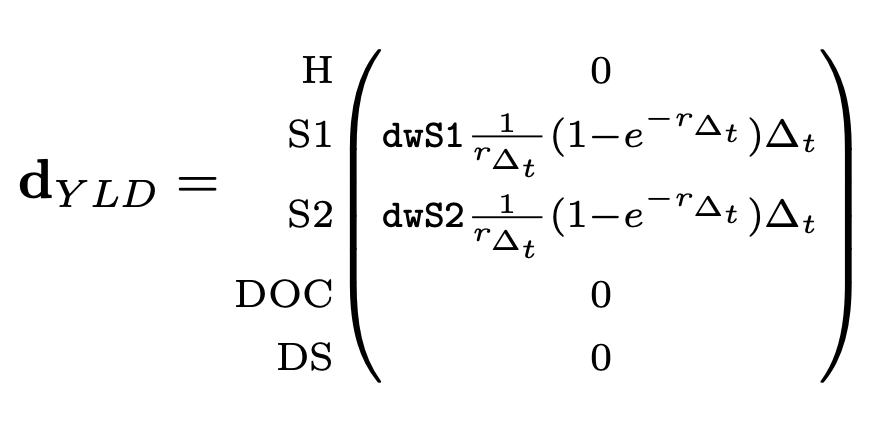
\includegraphics[width=0.4\textwidth,height=\textheight]{images/d_yld.png}
\end{center}

where \(\texttt{dwS1}\) and \(\texttt{dwS2}\) are the disability weights
for the Sick and Sicker states, respectively. In addition,
\(r_{\Delta_t}\) is the cycle discount rate, which is calculated as,

\begin{equation}\phantomsection\label{eq-cycledisc}{
r_{\Delta_t} = r \Delta_t
}\end{equation} where \(r\) is the annual discount rate and \(\Delta_t\)
is the cycle length.

In the YLD payoff vector, the term
\(\frac{1}{r_{\Delta_t}}(1-e^{-r_{\Delta_t}})\) is included as a
continuous-time discounting factor for the defined time step
\(\Delta_t\). This term is included to discount time \emph{within} each
cycle in order to maintain the continuous-time discounting approach used
in the original GBD equations (Larson, 2013).\footnote{Common
  discounting formulas, such as the discrete time discount factor
  \(\frac{1}{(1+r)^t}\), as well as the continuous time discount factor
  \(e^{-rt}\), are designed for a series of discrete ``payoffs'' at
  specific time points. By comparison, the continuous time discounting
  used in the GBD DALY equations (Equation~\ref{eq-yld} and
  Equation~\ref{eq-yll}) is based on an assumption that payffs accrue in
  a continuous stream. The discount adjustment factor shown here
  (\(\frac{1}{r}(1-e^{-rt})\))---and introduced in Larson
  (2013))---essentially ``smooths out'' the discrete YLD weight applied
  in each cycle to reflect this continuous flow. We have verified that
  application of this factor in our approach exactly replicate the
  example results using the GBD equations in Fox-Rushby \& Hanson
  (2001); see the Supplementary Appendix for these examples and code.}

To fully discount outcomes, we still must discount all future outcome
values back to baseline (\(t=0\)). Discounted years of life lost to
disability (YLD) at cycle \(t\) is given by

\begin{equation}\phantomsection\label{eq-yldt}{
YLD_t=\mathbf{s}'_0 \mathbf{P}_1\mathbf{P}_2\dots\mathbf{P}_t \mathbf{d}_{YLD}  \times{e^{-r_{\Delta_t} t}}
}\end{equation}

Total discounted YLDs are obtained by summing cycle-specific discounted
YLD outcomes,

\begin{equation}\phantomsection\label{eq-yldcum}{
YLD=\sum_{t=0}^{\omega-1} YLD_t
}\end{equation}

We can incorporate additional cycle adjustments (e.g., half-cycle
adjustment or an adjustment based on Simpson's rule) by defining a
adjustment factor \(c_t\) that multiplies the cycle-specific discounting
factor (i.e., \(e^{-r_{\Delta_t} t}\)) with other cycle-specific
adjustment values,

\begin{equation}\phantomsection\label{eq-yldcum2}{
YLD=\sum_{t=0}^{\omega-1} YLD(t)=\sum_{t=0}^{\omega-1}\left(\mathbf{s}'_0 \mathbf{P}_1\mathbf{P}_2\dots\mathbf{P}_t \mathbf{d}_{YLD}  \times c_t \right)
}\end{equation} where, at a minimum, \(c_t=e^{-r\Delta_t t}\) and can
also include any other cycle-correction value (e.g., 0.5 for half-cycle
correction or a Simpson's rule coefficient, etc.).

Finally, an equivalent way to calculate YLD outcomes is through matrix
multiplication of the Markov trace matrix and the YLD payoff vector,

\begin{equation}\phantomsection\label{eq-yldtrace}{
YLD = \sum_{t=0}^{\omega-1} \mathbf{S}\mathbf{d}_{YLD} \odot \mathbf{c}
}\end{equation} where \(\mathbf{c}\) is an \(\omega \times 1\) vector of
cycle discoutning/correction factors \(c_t\) and \(\odot\) is the
element-wise multiplication (Hadamard product) operator.

\subsubsection{Years of Life Lost to Disease (YLLs): Approach
1}\label{years-of-life-lost-to-disease-ylls-approach-1}

As noted in Section~\ref{sec-background} and in Equation~\ref{eq-yll},
YLLs are based on the present value of remaining life expectancy among
disease-related deaths. In a discrete time Markov model, these deaths
may occur in any cycle---though, like YLDs, the fully-discounted value
is calculated relative to baseline (\(t=0\)).

Define \(a_{t}\) as the age of the cohort at cycle \(t\), i.e.,

\begin{equation}\phantomsection\label{eq-aget}{
a_t = a_0 +t \cdot \Delta_t 
}\end{equation} where \(a_0\) is the age of the cohort at \(t=0\).

We next define \(Ex_t\) as the present value of remaining life
expectancy of the cohort in cycle \(t\).

Following the GBD discounting approach, \(Ex_{t}\) is given by

\begin{equation}\phantomsection\label{eq-pvEx}{
Ex_{t} = \frac{1}{r}\big (1 - e^{-rEx(a_{t})} \big )
}\end{equation}

where \(Ex(a_t)\) is the remaining life expectancy at age \(a\).
\(Ex(a_t)\) is drawn from either an exogenous (reference) life table, or
an endogenous life table, depending on the objectives of the modeling
exercise (Anand \& Reddy, 2019).

To calculate YLLs, we use the Markov trace to calculate \(m_t\), the
total number of new deaths from disease-related causes in each cycle. We
calculate \(m_t\) by taking the difference in state occupancy in the
disease-related death column (\texttt{DS}) in adjacent cycles. As above,
we can incorporate additional discounting and cycle adjustments into a
cycle correction term \(c_t\) and calculate total discounted (and
cycle-corrected) YLLs as

\begin{equation}\phantomsection\label{eq-yllt1}{
YLL_t=m_t Ex_t  \times{c_t} 
}\end{equation}

Total discounted YLLs are given by,

\begin{equation}\phantomsection\label{eq-yllcum1}{
YLL=\sum_{t=1}^{\omega-1} YLL_t = \sum_{t=1}^{\omega-1}m_t Ex_{t}  \times{c_t} 
}\end{equation}

\subsubsection{Years of Life Lost to Disease (YLLs): Approach
2}\label{years-of-life-lost-to-disease-ylls-approach-2}

YLLs under Approach 2 can be calculated in a similar way as YLDs, since
we have augmented the model with a transition tracking state that
directly etimates new deaths in each cycle. Define the YLL payoff vector
\(\mathbf{d}_{YLL,t}\), which has value \(Ex_{t}\) for the transition
tracker health state (\texttt{trDS}) and zeros elsewhere,

\begin{center}
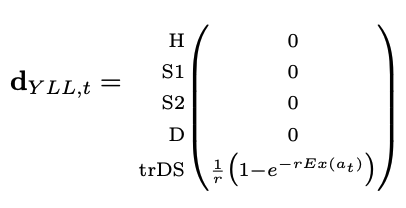
\includegraphics[width=0.4\textwidth,height=\textheight]{images/d_yll.png}
\end{center}

We can now apply similar equations as used for YLD outcomes to calculate
fully discounted YLLs,

\begin{equation}\phantomsection\label{eq-yllcum}{
YLL=\sum_{t=0}^{\omega-1} YLD(t)=\sum_{t=0}^{\omega-1}\left(\mathbf{s}'_0 \mathbf{P}_1\mathbf{P}_2\dots\mathbf{P}_t \mathbf{d}_{YLL,t}  \times c_t \right)
}\end{equation}

Alternatively, using the Markov trace, we stack each \(k \times 1\)
payoff vector (using \(\mathbf{d}_{YLL,t}^\top\) as rows) into an
\(\omega \times k\) payoff matrix \(\mathbf{D}\), and obtain total
adjusted YLLs as

\begin{equation}\phantomsection\label{eq-ylltrace}{
YLL = \sum_{t=0}^{\omega-1} \text{sum}(\mathbf{S} \odot \mathbf{D}) \odot \mathbf{c}
}\end{equation} where the \(\text{sum}()\) operator sums each row across
the \(k\) columns that result from \(\mathbf{S} \odot \mathbf{D}\).

\textsubscript{Source:
\href{https://graveja0.github.io/dalys/index.qmd.html}{Article
Notebook}}

\textsubscript{Source:
\href{https://graveja0.github.io/dalys/index.qmd.html}{Article
Notebook}}

\subsection{DALY Outcomes Under Approach 3}\label{sec-outcomes3}

Our advanced approach draws on Markov chain with rewards methods that
define reward matrices for occupancy-based (YLD) and transition-based
(YLL) outcomes. These reward matrices allow us to estimate outcomes for
any combination of health states and/or ages. Reward matrices have
notation \(\mathbf{R}_m\), where \(m\) indexes the moment of interest
(e.g., expected value, variance, etc.). We focus here on expected
outcomes (i.e., outcomes based on \(\mathbf{R}_1\))---though equations
are available to estimate higher-order moments and objects such as
variance, skewness, the coefficient of variation, etc.

\subsubsection{Years of Life Lived With Disease
(YLD)}\label{years-of-life-lived-with-disease-yld}

To calculate occupancy-based outcomes such as YLDs, we first define a
\(\tau \times \omega\) reward matrix \(\mathbf{H}\), which has
dimensions \(\tau \times \omega\) and is structured as shown in
Figure~\ref{fig-H-le}:

\begin{figure}

\centering{

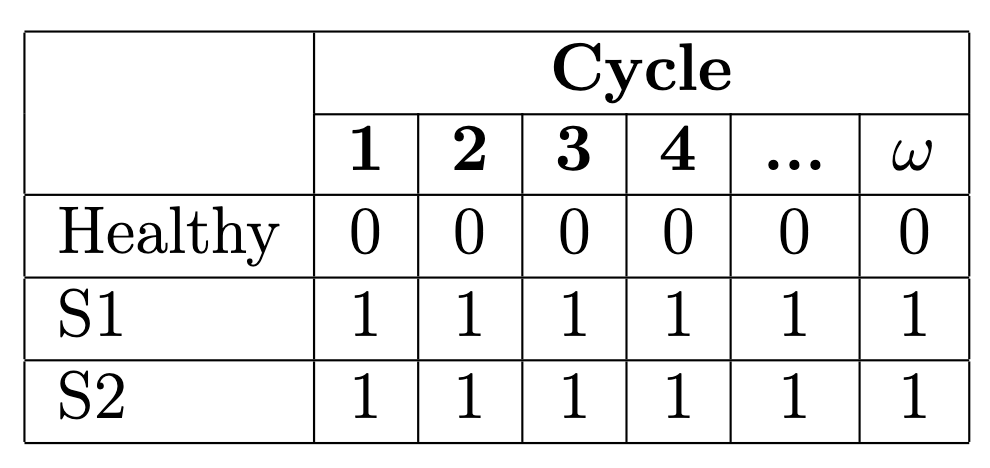
\includegraphics[width=0.4\textwidth,height=\textheight]{images/H-LE.png}

}

\caption{\label{fig-H-le}YLD reward matrix \(\mathbf{H}\)}

\end{figure}%

Cell values within this matrix can be set to one if we want to
potentially ``reward'' that health state-age combination in our outcome
measure, and zero otherwise.

We use this matrix to define the reward vector
\(\mathbf{h}\):\footnote{The \(\text{vec}\) operator stacks the columns
  of an \(m \times n\) matrix into a \(mn \times 1\) vector.}

\[
\mathbf{h} = \text{vec } \mathbf{H}
\] We also define \(\neg \mathbf{h}\) as the complement of
\(\mathbf{h}\), (i.e., values of 1.0 become 0, and vice versa).

We next define additional matrix \(\mathbf{V}\), which has the same
structure as \(\mathbf{H}\) but includes the (fully discounted)
disability weight:

\begin{figure}

\centering{

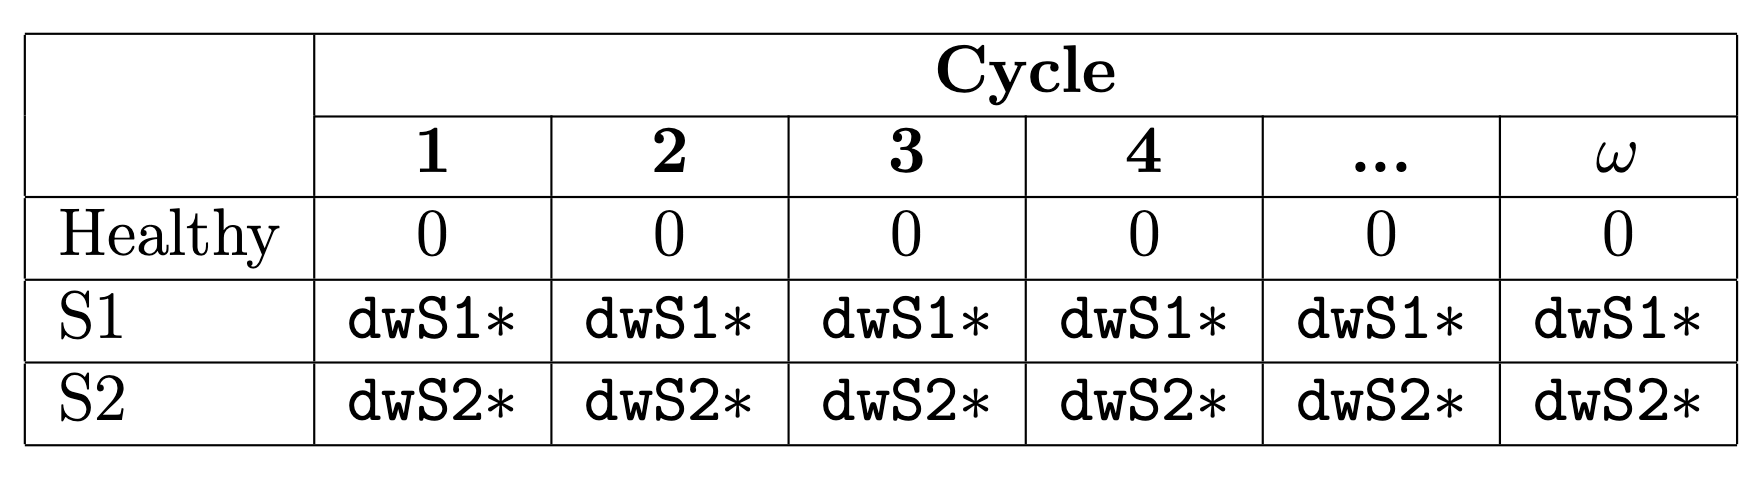
\includegraphics[width=0.6\textwidth,height=\textheight]{images/H-YLD.png}

}

\caption{\label{fig-H-yld}YLD reward matrix \(\mathbf{V}\)}

\end{figure}%

where
\(\texttt{dwS1}* = \texttt{dwS1} \times \Delta_t  \times  \frac{1}{r_{\Delta_t}}(1-e^{-r_{\Delta_t}}) \times e^{-r_{\Delta_t} t}\),
etc.

We similarly define an occupancy indicator vector \(\mathbf{v}\) just as
we did for \(\mathbf{h}\):

\[
\mathbf{v}_{m}=\operatorname{vec} \mathbf{V}_{m}
\]

\paragraph{Partial Occupancy}\label{partial-occupancy}

Because we are modeling a continuous-time disease progression progress
in discrete time, it is useful to make corrections for partial occupancy
in a cycle. Similar to a half-cycle correction often used in health
economic applications, the Markov chain with rewards approach does so by
assuming transitions occur half-way through a cycle. We operationalize
this assumption by defining,

\[
\begin{aligned}
\widetilde{\mathbf{B}}_{1} & =\mathbf{h} \mathbf{v}_{1}^{\top}+\frac{1}{2}(\neg \mathbf{h})\left(\mathbf{v}_{1}^{\top}\right)+\frac{1}{2}\left(\mathbf{v}_{1}\right)\left(\neg \mathbf{h}^{\top}\right) \\
\end{aligned}
\] and

\[
\widetilde{\mathbf{C}}_{1}=\frac{1}{2} \mathbf{1}_{\alpha} \mathbf{v_1}^{\top}
\] where \(\mathbf{1}_{\alpha}\) is a vector of ones with length
\(\alpha\).

We combine \(\widetilde{\mathbf{B}}_{1}\) and
\(\widetilde{\mathbf{C}}_{1}\) to obtain:

\[
\widetilde{\mathbf{R}}^{YLD}_{1}=\left(\begin{array}{c|c}
\widetilde{\mathbf{B}}_{1} & \mathbf{0} \\
\hline \widetilde{\mathbf{C}}_{1} & \mathbf{0}
\end{array}\right) 
\] which has same block structure and dimensions as the transition
probability matrix \(\widetilde{\mathbf{P}}\)
(Equation~\ref{eq-Ptilde}).

\subsubsection{Years of Life Lost to Disease
(YLL)}\label{years-of-life-lost-to-disease-yll}

For transition-based outcomes such as YLLs, we define the first moment
of remaining life expectancy as the vector
\(\widetilde{\boldsymbol{\eta}}^{\top}\). This vector has dimensions
\(\tau\omega \times 1\) and has the following basic structure:

\[
\widetilde{\mathbf{\eta}}=\left(\begin{array}{c}
\eta_{11} \\
\vdots \\
\eta_{\tau 1} \\
\hline \vdots \\
\hline \eta_{1 \omega} \\
\vdots \\
\eta_{\tau \omega}
\end{array}\right)
\] where \(\eta_{i x}\) is remaining life expectancy for an individual
in health state \(i\) at a given age \(x\). In this structure, remaining
life expectancy for each health state is grouped within age classes.
Remaining life expectancy should also enter \(\eta_{i x}\) as fully
discounted back to \(t=0\).

We next construct the reward matrices:

\[
\begin{aligned}
\widetilde{\mathbf{B}}_{1} & =\left(\mathbf{0}_{\tau \omega \times \tau \omega}\right) \\
\widetilde{\mathbf{C}}_{1} & =\left(\begin{array}{c}
\widetilde{\boldsymbol{\eta}}_{1}^{\top} \\
\mathbf{0}_{1 \times \tau \omega}
\end{array}\right) .
\end{aligned}
\]

and

\[
\widetilde{\mathbf{R}}^{YLL}_{1}=\left(\begin{array}{c|c}
\mathbf{0}_{\tau \omega \times \tau \omega} & \mathbf{0}_{\tau \omega \times 2} \\
\hline \widetilde{\boldsymbol{\eta}}_{1}^{\top} & \mathbf{0}_{1 \times 2} \\
\mathbf{0}_{1 \times \tau \omega} & \mathbf{0}_{1 \times 2}
\end{array}\right)
\]

\subsubsection{Expected YLD and YLL
Outcomes}\label{expected-yld-and-yll-outcomes}

The expected value of outcome \(Y\) (where \(Y \in \{YLD, YLL\}\)) is
estimated by,

\begin{equation}\phantomsection\label{eq-app3out}{
\begin{aligned}
& \widetilde{\boldsymbol{\rho}}^{Y}_{1}=\widetilde{\mathbf{N}}^{\top} \mathbf{Z}\left(\widetilde{\mathbf{P}} \odot \widetilde{\mathbf{R}}^Y_{1}\right)^{\top} \mathbf{1}_{s} 
\end{aligned}
}\end{equation} where \(\widetilde{\mathbf{N}}\) is the fundamental
matrix,

\[
\widetilde{\mathbf{N}}=(\mathbf{I}-\widetilde{\mathbf{U}})^{-1}
\] and \(\mathbf{Z}\) is

\[
\mathbf{Z}=\left(\mathbf{I}_{\tau \omega} \mid \mathbf{0}_{\tau \omega \times \alpha}\right)
\]

Total (across all ages) outcomes for each starting health state are
calculated as

\begin{equation}\phantomsection\label{eq-app3outstate}{
\boldsymbol{\rho}_{1}^{Y,\text {stage }}(\operatorname{cycle} t)=\left(\mathbf{e}_{t}^{\top} \otimes \mathbf{I}_{\tau}\right) \widetilde{\boldsymbol{\rho}}^Y_{1} \quad \tau \times 1
}\end{equation} where \(\otimes\) is the Kronecker operator and
\(\mathbf{e}_{t}\) is a vector of length \(\omega\) with a value of one
in the first position and zero elsewhere; this facilitates calculating
expected outcomes from the baseline period (i.e., \(t=0\)).

Alternatively, we may wish to calculate outcomes separately under
different starting ages, and for a specified starting health state
(e.g., healthy). This is given by

\begin{equation}\phantomsection\label{eq-app3outage}{
\boldsymbol{\rho}_{1}^{Y,\text {age }}(\text { stage } i)=\left(\mathbf{I}_{\omega} \otimes \mathbf{e}_{i}^{\top}\right) \widetilde{\boldsymbol{\rho}}^Y_{1} \quad \omega \times 1,
}\end{equation} where \(\mathbf{e}_{i}\) is a vector of length \(\tau\)
with a value of one in the initial health state position of interest
(e.g., \texttt{Healthy}) and zero elsewhere.

\textsubscript{Source:
\href{https://graveja0.github.io/dalys/index.qmd.html}{Article
Notebook}}

\subsection{Results}\label{sec-results}

Table~\ref{tbl-trace1} shows the Markov trace for the first five cycles
under Approach 1, while Table~\ref{tbl-trace2} shows the trace under
Approach 2. Table~\ref{tbl-trace1} also includes a new column
(\texttt{deaths\_disease}) that is calculated as the difference in state
occupancy in the \texttt{DS} column between cycles. This extra step will
be necessary later for calculating YLL outcomes. The trace shown under
Approach 2 (Table~\ref{tbl-trace2}), by comparison, automatically
calculates new deaths through the inclusion of the transition state
\texttt{trDS}; the values under \texttt{deaths\_disease} and
\texttt{trDS} are identical, again highlighting that either approach can
be used to calculate the number of disease-related deaths in each cycle.

\begin{table}

\caption{\label{tbl-trace1}Markov Trace Under Approach 1}

\centering{

\begin{tabular}{r|r|r|r|r|r|r}
\hline
cycle & H & S1 & S2 & DOC & DS & deaths\_disease\\
\hline
0 & 1.0000 & 0.0000 & 0.0000 & 0.0000 & 0.0000 & 0.0000\\
\hline
1 & 0.8870 & 0.1046 & 0.0062 & 0.0020 & 0.0003 & 0.0003\\
\hline
2 & 0.8232 & 0.1521 & 0.0197 & 0.0040 & 0.0010 & 0.0008\\
\hline
3 & 0.7832 & 0.1723 & 0.0363 & 0.0060 & 0.0022 & 0.0012\\
\hline
4 & 0.7547 & 0.1796 & 0.0540 & 0.0080 & 0.0037 & 0.0015\\
\hline
5 & 0.7321 & 0.1808 & 0.0717 & 0.0099 & 0.0056 & 0.0019\\
\hline
\end{tabular}

}

\end{table}%

\textsubscript{Source:
\href{https://graveja0.github.io/dalys/index.qmd.html}{Article
Notebook}}

\begin{table}

\caption{\label{tbl-trace2}Markov Trace Under Approach 2}

\centering{

\begin{tabular}{r|r|r|r|r|r}
\hline
cycle & H & S1 & S2 & D & trDS\\
\hline
0 & 1.0000 & 0.0000 & 0.0000 & 0.0000 & 0.0000\\
\hline
1 & 1.0000 & 0.0000 & 0.0000 & 0.0000 & 0.0000\\
\hline
2 & 0.8870 & 0.1046 & 0.0062 & 0.0023 & 0.0003\\
\hline
3 & 0.8232 & 0.1521 & 0.0197 & 0.0050 & 0.0008\\
\hline
4 & 0.7832 & 0.1723 & 0.0363 & 0.0082 & 0.0012\\
\hline
5 & 0.7547 & 0.1796 & 0.0540 & 0.0117 & 0.0015\\
\hline
\end{tabular}

}

\end{table}%

\textsubscript{Source:
\href{https://graveja0.github.io/dalys/index.qmd.html}{Article
Notebook}}

\begin{table}
\centering
\begin{tabular}{l|r|r|r|r|r|r|r|r}
\hline
Scenario & Life-Years & YLDs & YLLs & DALYs & DALY-Hack & QALY-like DALY & QALY & Costs\\
\hline
\multicolumn{9}{l}{\textbf{Approaches 1 and 2 (Markov Trace)}}\\
\hline
\hspace{1em}SoC & 86.567 & 4.608 & 2.683 & 7.291 & 9.624 & 21.872 & 21.872 & 158566.1\\
\hline
\hspace{1em}A & 86.567 & 3.901 & 2.683 & 6.584 & 8.917 & 22.590 & 22.590 & 292352.4\\
\hline
\hspace{1em}B & 103.352 & 3.820 & 2.028 & 5.847 & 7.741 & 23.699 & 23.699 & 255608.1\\
\hline
\hspace{1em}AB & 103.352 & 2.953 & 2.028 & 4.981 & 6.875 & 24.579 & 24.579 & 375043.1\\
\hline
\multicolumn{9}{l}{\textbf{Approach 3 (Markov Chain With Rewards)}}\\
\hline
\hspace{1em}SoC & 86.644 & 4.637 & 2.810 & 7.447 &  &  & 22.309 & 158365.5\\
\hline
\hspace{1em}A & 86.644 & 3.896 & 2.810 & 6.706 &  &  & 23.024 & 291128.7\\
\hline
\hspace{1em}B & 103.717 & 3.844 & 2.124 & 5.969 &  &  & 24.142 & 254886.6\\
\hline
\hspace{1em}AB & 103.717 & 2.949 & 2.124 & 5.074 &  &  & 25.019 & 373515.0\\
\hline
\end{tabular}
\end{table}

\textsubscript{Source:
\href{https://graveja0.github.io/dalys/index.qmd.html}{Article
Notebook}}

\begin{table}
\centering
\begin{tabular}{l|r|r|r|r|r|l}
\hline
Strategy & Cost & Effect & Inc\_Cost & Inc\_Effect & ICER & Status\\
\hline
\multicolumn{7}{l}{\textbf{QALY - Approaches 1 \& 2}}\\
\hline
\hspace{1em}SoC & 158566 & 21.872 &  &  &  & \vphantom{1} ND\\
\hline
\hspace{1em}B & 255608 & 23.699 & 97042 & 1.827 & 53119 & \vphantom{1} ND\\
\hline
\hspace{1em}AB & 375043 & 24.579 & 119435 & 0.879 & 135813 & \vphantom{1} ND\\
\hline
\hspace{1em}A & 292352 & 22.590 &  &  &  & \vphantom{1} D\\
\hline
\multicolumn{7}{l}{\textbf{QALY - Approach 3}}\\
\hline
\hspace{1em}SoC & 158365 & 22.309 &  &  &  & ND\\
\hline
\hspace{1em}B & 254887 & 24.142 & 96521 & 1.833 & 52656 & ND\\
\hline
\hspace{1em}AB & 373515 & 25.019 & 118628 & 0.877 & 135271 & ND\\
\hline
\hspace{1em}A & 291129 & 23.024 &  &  &  & D\\
\hline
\multicolumn{7}{l}{\textbf{DALY - Approaches 1 \& 2}}\\
\hline
\hspace{1em}SoC & 158566 & 7.291 &  &  &  & ND\\
\hline
\hspace{1em}B & 255608 & 5.847 & 97042 & 1.444 & 67203 & ND\\
\hline
\hspace{1em}AB & 375043 & 4.981 & 119435 & 0.866 & 137860 & ND\\
\hline
\hspace{1em}A & 292352 & 6.584 &  &  &  & D\\
\hline
\multicolumn{7}{l}{\textbf{DALY - Approach 3}}\\
\hline
\hspace{1em}SoC & 158365 & 7.447 &  &  &  & ND\\
\hline
\hspace{1em}B & 254887 & 5.969 & 96521 & 1.478 & 65287 & ND\\
\hline
\hspace{1em}AB & 373515 & 5.074 & 118628 & 0.895 & 132583 & ND\\
\hline
\hspace{1em}A & 291129 & 6.706 &  &  &  & D\\
\hline
\multicolumn{7}{l}{\textbf{DALY-Hack}}\\
\hline
\hspace{1em}SoC & 158566 & 9.624 &  &  &  & ND\\
\hline
\hspace{1em}B & 255608 & 7.741 & 97042 & 1.883 & 51524 & ND\\
\hline
\hspace{1em}AB & 375043 & 6.875 & 119435 & 0.866 & 137860 & ND\\
\hline
\hspace{1em}A & 292352 & 8.917 &  &  &  & D\\
\hline
\multicolumn{7}{l}{\textbf{QALY-like DALY}}\\
\hline
\hspace{1em}SoC & 158566 & 21.872 &  &  &  & ND\\
\hline
\hspace{1em}B & 255608 & 23.699 & 97042 & 1.827 & 53119 & ND\\
\hline
\hspace{1em}AB & 375043 & 24.579 & 119435 & 0.879 & 135813 & ND\\
\hline
\hspace{1em}A & 292352 & 22.590 &  &  &  & D\\
\hline
\end{tabular}
\end{table}

\textsubscript{Source:
\href{https://graveja0.github.io/dalys/index.qmd.html}{Article
Notebook}}

\textsubscript{Source:
\href{https://graveja0.github.io/dalys/index.qmd.html}{Article
Notebook}}

\subsection{Conclusion}\label{conclusion}

\subsection{To Incorporate}\label{to-incorporate}

\begin{itemize}
\tightlist
\item
  \href{https://academic.oup.com/heapol/article/21/5/402/578296?login=false}{Link}
\item
  \href{https://link.springer.com/article/10.1007/s40258-022-00722-3}{Link}
  \#\# References \{.unnumbered\}
\end{itemize}

\phantomsection\label{refs}
\begin{CSLReferences}{1}{0}
\vspace{1em}

\bibitem[\citeproctext]{ref-alarid2023introductory}
Alarid-Escudero, F., Krijkamp, E., Enns, E. A., Yang, A., Hunink, M. M.,
Pechlivanoglou, P., \& Jalal, H. (2023). An introductory tutorial on
cohort state-transition models in r using a cost-effectiveness analysis
example. \emph{Medical Decision Making}, \emph{43}(1), 3--20.

\bibitem[\citeproctext]{ref-anand2019}
Anand, S., \& Reddy, S. G. (2019). The Construction of the DALY:
Implications and Anomalies. \emph{SSRN Electronic Journal}.
\url{https://doi.org/10.2139/ssrn.3451311}

\bibitem[\citeproctext]{ref-bertram2021}
Bertram, M. Y., Lauer, J. A., Stenberg, K., \& Edejer, T. T. T. (2021).
Methods for the Economic Evaluation of Health Care Interventions for
Priority Setting in the Health System: An Update From WHO CHOICE.
\emph{International Journal of Health Policy and Management}.
\url{https://doi.org/10.34172/ijhpm.2020.244}

\bibitem[\citeproctext]{ref-caswell2021a}
Caswell, H., \& van Daalen, S. (2021). Healthy longevity from
incidence-based models: More kinds of health than stars in the sky.
\emph{Demographic Research}, \emph{45}, 397--452.
\url{https://doi.org/10.4054/demres.2021.45.13}

\bibitem[\citeproctext]{ref-caswell2018}
Caswell, H., \& Zarulli, V. (2018). Matrix methods in health demography:
a new approach to the stochastic analysis of healthy longevity and
DALYs. \emph{Population Health Metrics}, \emph{16}(1).
\url{https://doi.org/10.1186/s12963-018-0165-5}

\bibitem[\citeproctext]{ref-Feng2020}
Feng, X., Kim, D. D., Cohen, J. T., Neumann, P. J., \& Ollendorf, D. A.
(2020). Using QALYs versus DALYs to measure cost-effectiveness: How much
does it matter? \emph{International Journal of Technology Assessment in
Health Care}, \emph{36}(2), 96--103.
\url{https://doi.org/10.1017/s0266462320000124}

\bibitem[\citeproctext]{ref-rushby2001}
Fox-Rushby, J., \& Hanson, K. (2001). Calculating and presenting
disability adjusted life years (DALYs) in cost-effectiveness analysis.
\emph{Health Policy and Planning}, \emph{16}(3), 326--331.
\url{https://doi.org/10.1093/heapol/16.3.326}

\bibitem[\citeproctext]{ref-globalburdenofdiseasecollaborativenetwork2021}
Global Burden of Disease Collaborative Network. (2021). Global burden of
disease study 2019 (GBD 2019) reference life table. Institute for Health
Metrics; Evaluation (IHME). \url{https://doi.org/10.6069/1D4Y-YQ37}

\bibitem[\citeproctext]{ref-graves2021}
Graves, J., Garbett, S., Zhou, Z., Schildcrout, J. S., \& Peterson, J.
(2021). Comparison of Decision Modeling Approaches for Health Technology
and Policy Evaluation. \emph{Medical Decision Making}, \emph{41}(4),
453--464. \url{https://doi.org/10.1177/0272989x21995805}

\bibitem[\citeproctext]{ref-henderson1981}
Henderson, H. V., \& Searle, S. R. (1981). The vec-permutation matrix,
the vec operator and Kronecker products: a review. \emph{Linear and
Multilinear Algebra}, \emph{9}(4), 271--288.
\url{https://doi.org/10.1080/03081088108817379}

\bibitem[\citeproctext]{ref-iosifescu1980}
Iosifescu, M. (1980). Finite markov processes and their applications.
wiley. \emph{New York}.

\bibitem[\citeproctext]{ref-larson2013calculating}
Larson, B. A. (2013). Calculating disability-adjusted-life-years lost
(DALYs) in discrete-time. \emph{Cost Effectiveness and Resource
Allocation}, \emph{11}(1), 1--6.

\bibitem[\citeproctext]{ref-Murray1997}
Murray, C. J., \& Lopez, A. D. (1997). Mortality by cause for eight
regions of the world: Global Burden of Disease Study. \emph{The Lancet},
\emph{349}(9061), 1269--1276.
\url{https://doi.org/10.1016/s0140-6736(96)07493-4}

\bibitem[\citeproctext]{ref-murray2020}
Murray, C. J. L., Aravkin, A. Y., Zheng, P., Abbafati, C., Abbas, K. M.,
Abbasi-Kangevari, M., et al. (2020). Global burden of 87 risk factors in
204 countries and territories, 1990{\textendash}2019: a systematic
analysis for the Global Burden of Disease Study 2019. \emph{The Lancet},
\emph{396}(10258), 1223--1249.
\url{https://doi.org/10.1016/s0140-6736(20)30752-2}

\bibitem[\citeproctext]{ref-sassi2006calculating}
Sassi, F. (2006). Calculating QALYs, comparing QALY and DALY
calculations. \emph{Health Policy and Planning}, \emph{21}(5), 402--408.

\bibitem[\citeproctext]{ref-who2020methods}
WHO, G. (2013). WHO methods and data sources for global burden of
disease estimates 2000--2019. \emph{Geneva: Department of Health
Statistics and Information Systems}. Retrieved from
\url{https://cdn.who.int/media/docs/default-source/gho-documents/global-health-estimates/ghe2019_daly-methods.pdf}

\bibitem[\citeproctext]{ref-Wilkinson2016}
Wilkinson, T., Sculpher, M. J., Claxton, K., Revill, P., Briggs, A.,
Cairns, J. A., et al. (2016). The International Decision Support
Initiative Reference Case for Economic Evaluation: An Aid to Thought.
\emph{Value in Health}, \emph{19}(8), 921--928.
\url{https://doi.org/10.1016/j.jval.2016.04.015}

\end{CSLReferences}



\end{document}
